% Author: Bhishan Poudel
% Date  :
% Update:
%
%
%#*******************************************************
%#=======================================================
%# Chapter 3: PSF Creation Using PhoSim
%#=======================================================
%#*******************************************************
%
%
\section{Chapter 3: PSF Creation Using PhoSim}\label{sec:chap3}
In case of galaxy fitting software \textbf{Galfit}, we created the PSF needed using an on-line tool called \textbf{TinyTim}. The PSF was specially designed for HST ACS Wide Field Camera observations. Here, we again want to create a general purpose PSF using a flat SED. SED stands for "Spectral Energy Distribution" which is simply a table of flux and wavelength. In our galaxy simulation program \textbf{Jedisim}, we use the PSF created by a program called '\textbf{PhoSim}'. PhoSim is a photon simulator application which uses Monte Carlo codes to calculate the physics of the atmosphere and the telescope \& camera optics. \footnote{$https://bitbucket.org/phosim/phosim_release/wiki/Home$}

To run \textbf{PhoSim}, we need a SED file, an instance catalog and a background file. Here, we are using flat SED file provided from SEDs list recommended from \textbf{PhoSim} website.
The plot of wavelength versus flux of flat sed is given below:
  \begin{figure}[ht!]
      \centering
      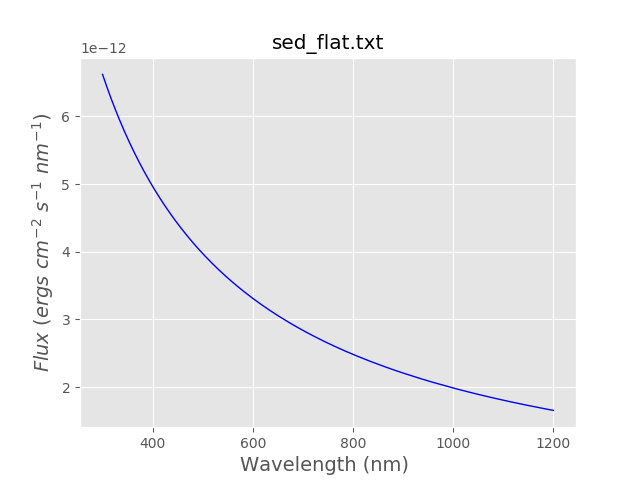
\includegraphics[width=0.5\textwidth]{sed_flat}
      \caption{Flat SED}
      \label{[fig:sed_flat]}
  \end{figure}

Here, the SED has flux values for wavelengths 400 to 1200 nanometers.
We are particularly interested only for the wavelength range of LSST r band filter. Looking at the file $phosim/data/lsst/filter\_2.txt$ and choosing only the range of the filter for transmission $>=5\%$ we get the range of 531 nm to 696 nm. From now on the range 531 nm to 696 nm will be called the
broadband range. We split this broadband into 21 equal parts and call each part a narrowband. For example, narrowband0 is from wavelength 5310 Angstrom to 5388 Angstrom. From these wavelengths we create 21 narrowband SED files and one broadband sed file. To get the psf using PHOSIM, we need three things: a sed file,an instance catalog, and a background file. We have got sed file from SEDs directory recommended by PhoSim, now we need to choose the background. For the background we chose a simple background file as shown below: 
\verbatiminput{seds/background1.txt}

 The third component needed is instance catalog file. The important parameters in an instance catalog are SIM\_SEED, SIM\_VISTIME, and object.
 The output PSF file will depend on the initial random seed to the PhoSim software. For the simplicity, we choose this seed number to be 1000. Similarly we choose the simulation time to be 5 minutes (equal to 300 seconds) as the SIM\_VISTIME parameter.
The "object" parameter consist of multiple fields. For example, we have used:
\begin{verbatim}
object 0 0.0 0.0 24 ../../../Research/psf_creation_phosim/scripts/
narrowband_seds/narrowband0.sed 0 0 0 0 0 0 star none none

These fields corresponds to following settings:
object ID RA DEC MAG_NORM SED_NAME REDSHIFT GAMMA1 GAMMA2 KAPPA DELTA_RA DELTA_DEC SOURCE_TYPE source_pars DUST_REST_NAME dust_pars_1 DUST_LAB_NAME dust_pars_1

The non-trivial components are magnitude of the star, name of the sed file used and source type (here, it is star).
\end{verbatim}
\footnote{https://bitbucket.org/phosim/phosim\_release/wiki/Instance\%20Catalog}
An example of instance catalog file can be found in PhoSim software
installation directory $phosim/examples/small\_catalog$.
An example of the instance catalog we used is given below: 
\verbatiminput{seds/narrowband0.txt}

The PHOSIM gives multiple outputs, out of which what we are interested in only the electron image named as $lsst\_e\_99999999\_f2\_R22\_S11\_E000.fits.gz$. For a given SED, we unzip this file and take as the psf file. Here for the broadband sed we got our psf for the broadband settings. However, the program \textbf{Jedisim} needs 21 narrowband psf images. To get these 21 narrowband psf images, we feed the 21 narrowband sed files to the PhoSim and get the required psf images. We take the middle narrowband psf i.e. psf10.fits as the monochromatic psf. We also normalize the total flux across all the psf images. This means, we first calculate the total flux of psf10.fits and scale the flux of all other psf images.

